% Chapter Template

\chapter{Scaffold} % Main chapter title

\label{Chapter7} % Change X to a consecutive number; for referencing this chapter elsewhere, use \ref{ChapterX}

 %----------------------------------------------------
 
 

Gli scaffold sono dei supporti tridimensionali che forniscono alle cellule un ambiente su cui aderire, differenziarsi e moltiplicarsi. L'ingegneria tissutale e gli scaffold si sono sviluppati con l'obiettivo di favorire la rigenerazione di tessuti danneggiati dell'organismo, in sostituzione a \emph{innesti autologhi} e \emph{trapianti da donatore}.\\ Gli innesti autologhi (ad esempio di cute o osso) richiedono un ulteriore intervento chirurgico per essere prelevati; inoltre il tessuto da prelevare potrebbe essere presente in quantità non sufficienti alle necessità di rigenerazione del sito danneggiato. Per quanta riguarda gli innesti omologhi (da donatore della stessa specie) le problematiche di maggior importanza riguardano la carenza di materiale da donatore e il rischio biologico di infezione e rigetto.\\
Per fornire il miglior ambiente ad ogni gruppo di cellule coltivato, sono stati descritti scaffold realizzati in una ampia varietà di materiali. Ogni tessuto è infatti unico per proprietà meccaniche e funzionali, oltre che per la sua micro e macrostruttura.\\ L'introduzione delle tecniche di manifattura additiva nella produzione di scaffold ha portato novità nei materiali usati e nelle combinazioni di questi, ed ha reso possibile l'esplorazione di design alternativi. Gli scaffold possono essere costituiti da polimeri biologici, da polimeri sintetici, da materiali ceramici e da combinazioni di questi \parencite{Reference128}.\\
La diffusione di cellule e nutrienti e la rimozione delle sostanze di scarto deve essere facilitata dalla struttura dello scaffold per favorire la sopravvivenza cellulare. La \emph{porosità} dello scaffold è quindi un parametro fondamentale, assieme all'\emph{interconnessione delle porosità}. Fattori di crescita e proteine regolatrici dell'adesione cellulare possono essere integrate negli scaffold, per agevolare la distribuzione delle cellule e regolarla nel caso di \emph{scaffold multifase} \parencite{Reference129}. Lo scaffold deve inoltre essere riassorbibile, ed il tasso di riassorbimento deve essere in accordo al tasso di rigenerazione del tessuto che si intende riparare; l'obiettivo degli scaffold è infatti quello di stimolare la rigenerazione completa del tessuto, con la totale scomparsa dello scaffold dal sito di impianto. \\
Tra gli scaffold usati più recentemente in ambito odontoiatrico troviamo sicuramente i granuli di materiali ceramici come \emph{fosfato tricalcico} (TCP, TriCalcium Phosphate), \emph{Idrossiapatite} (HA) ed MTA. Questi materiali sono usati per la rigenerazione dell'osso, assieme alle membrane in collagene o PTFE usate per compartimentalizzare il sito di innesto. I granuli ceramici formano una struttura porosa che viene tenuta insieme dal coagulo, favorendo la diffusione di cellule e nutrienti e stimolando la produzione di osso. \\ La composizione chimica di questi materiali granulari è simile a quella dell'osso, la superficie ad alta rugosità consente la stabilizzazione del coagulo, l'adsorbimento di fattori di crescita ed una aumentata adesione cellulare. La porosità dei materiali descritti non è però controllabile, perché dipende dall'aggregazione che si viene a creare durante la formazione del coagulo. Il coagulo risultante è inoltre instabile e inadatto a sostenere carichi meccanici durante le prime fasi di consolidamento \parencite{Reference131}. Il tasso di riassorbimento di alcuni di questi materiali è lento, per cui spesso si ritrovano per molto tempo nel sito.\\
L'utilizzo di scaffold tridimensionali ha quindi cercato di superare queste limitazioni, cercando di fornire una soluzione ottimale a queste problematiche e di aumentare la predicibilità del trattamento rigenerativo. L'introduzione della manifattura additiva ha reso possibile un maggiore controllo sull'architettura dello scaffold, portando a risultati molto incoraggianti \parencite{Reference136}, \parencite{Reference137}.\\
\begin{figure}[h]
\vspace{-10pt}
	\begin{center}
	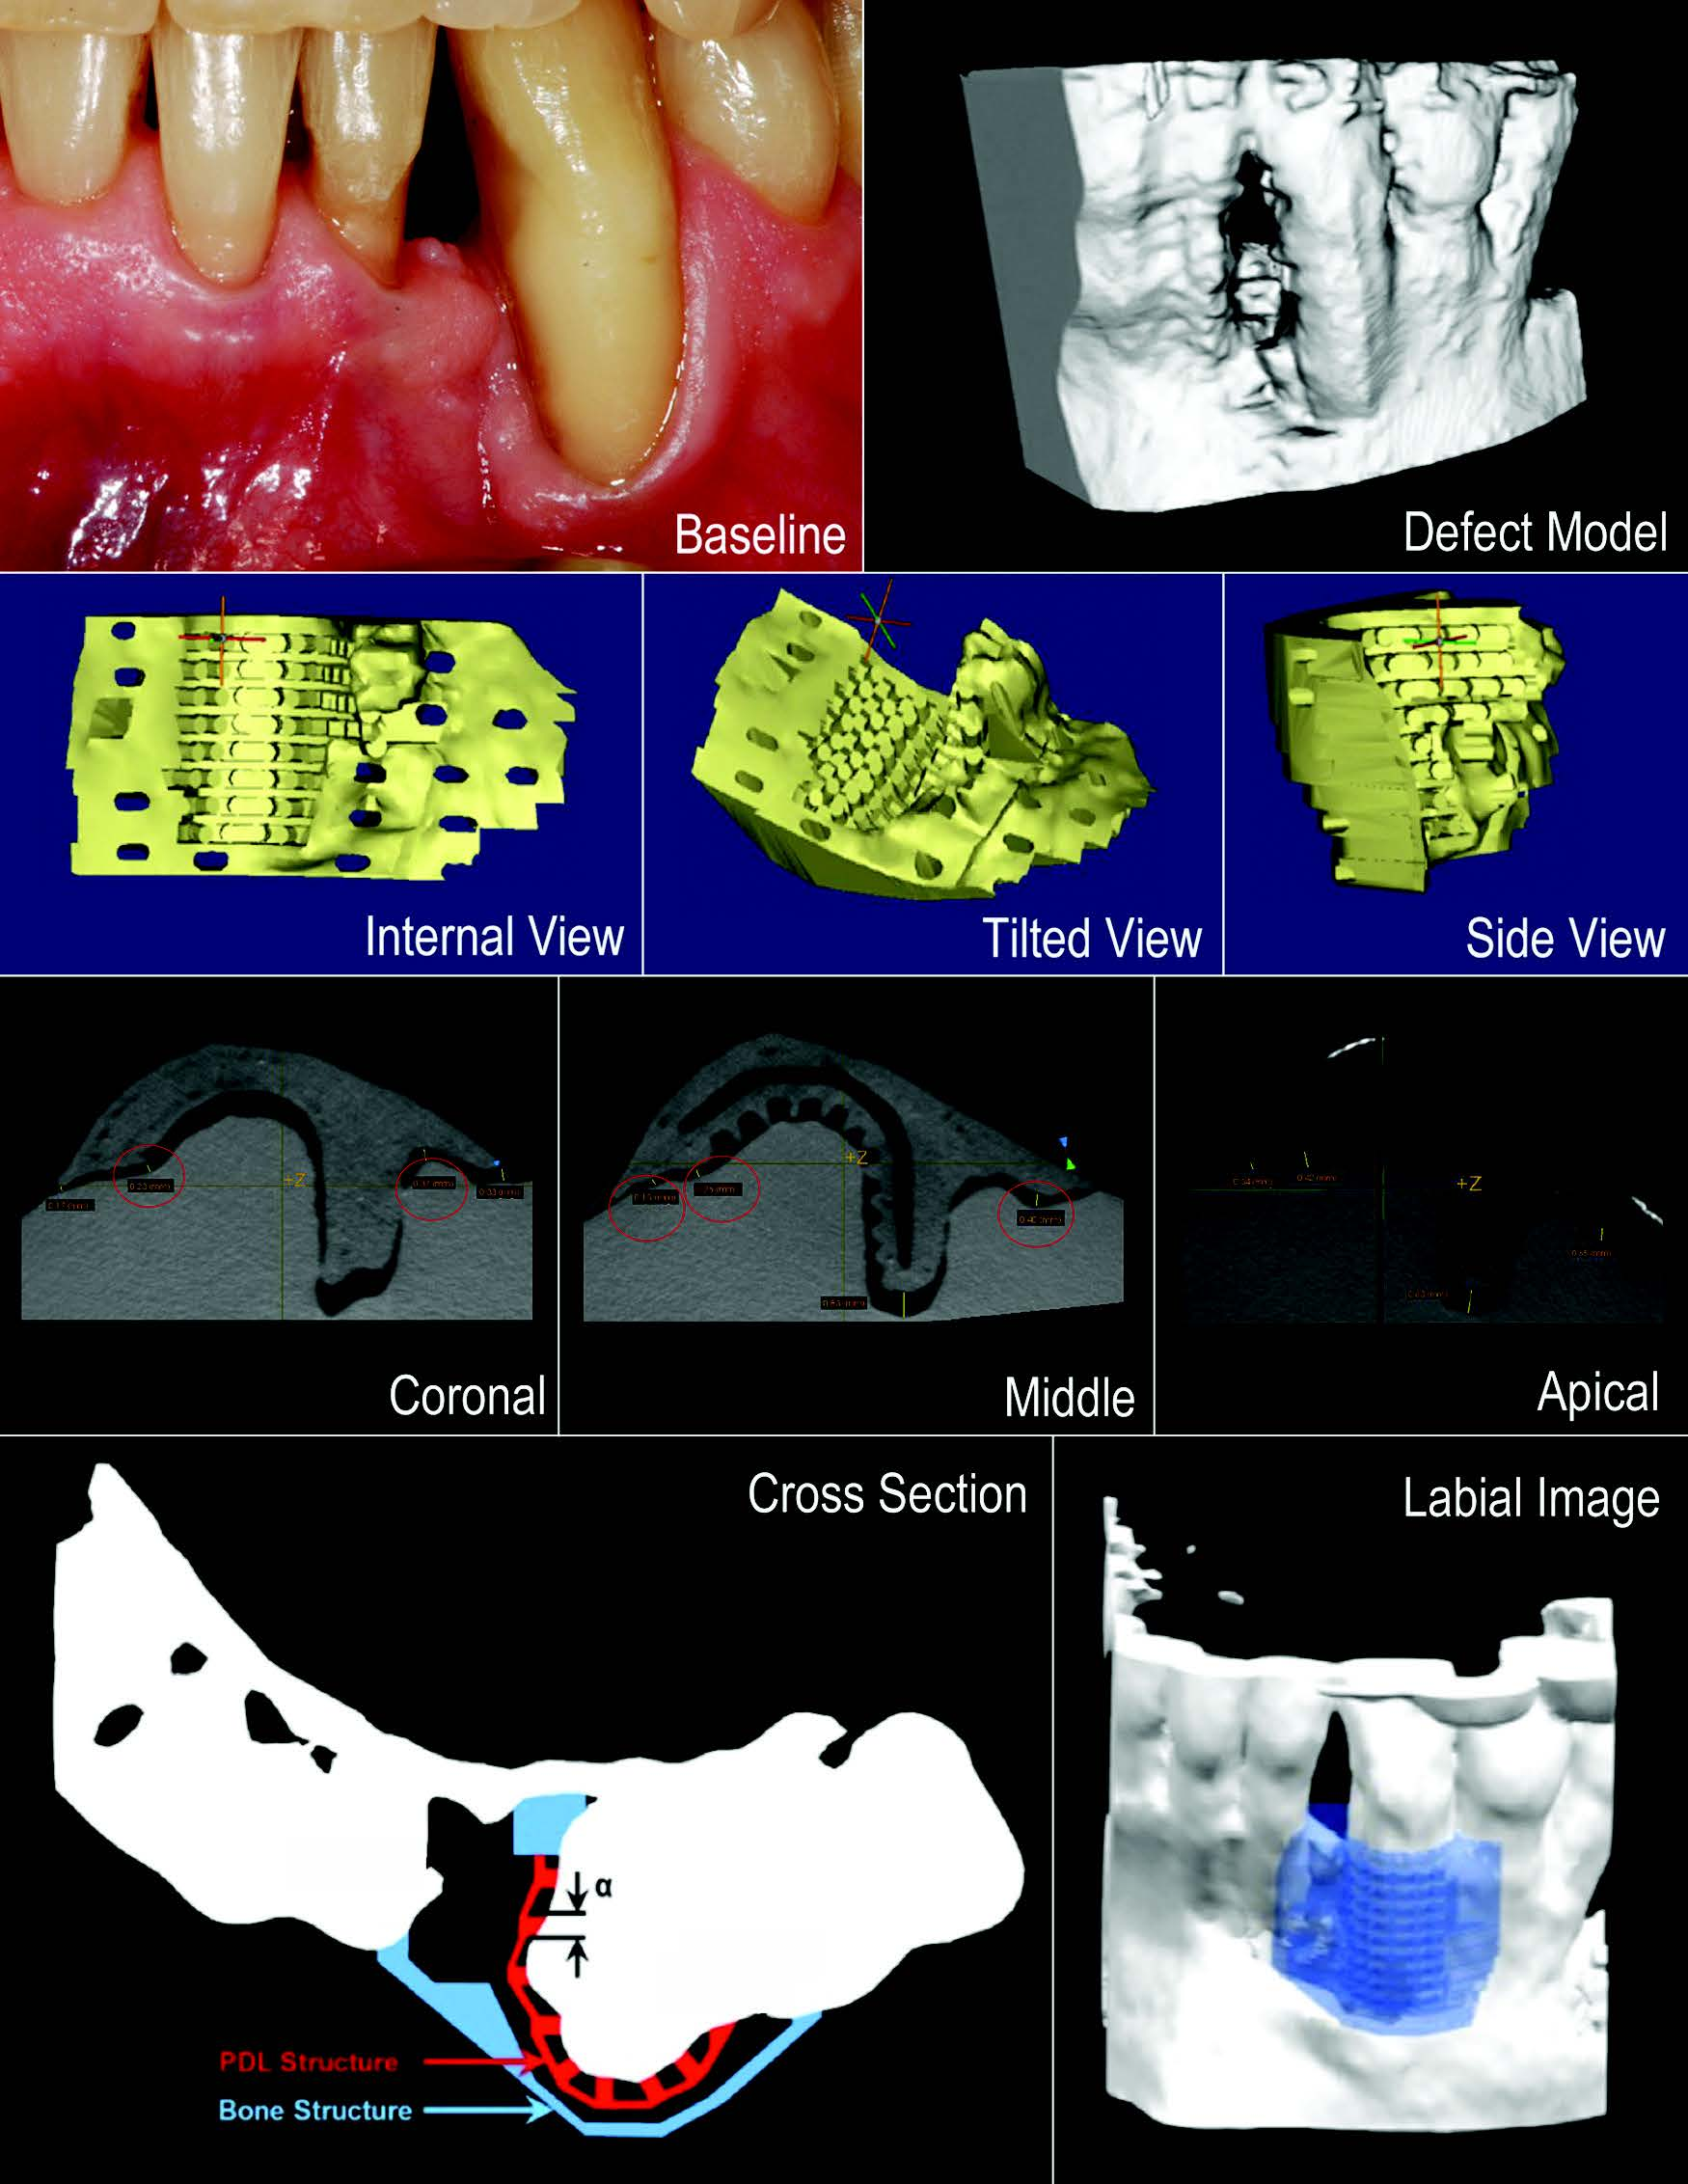
\includegraphics[width=0.6\textwidth, keepaspectratio]{scaf_paro}
    \caption{Scaffold per la rigenerazione parodontale realizzato da \emph{Rasperini et al} \parencite{Reference134}.}
    \label{fig:scaf_paro}
	\end{center}
\vspace{-20pt}
\end{figure}

Strutture in OCT (\emph{fosfato ottocalcico}) risultano \emph{\textbf{ostoinduttive}}, cioè stimolano le cellule alla differenziazione osteoblastica \parencite{Reference130}. Osteoinduttivo si è rivelato anche uno scaffold composito realizzato in Policaprolattone ed osso decellularizzato \parencite{Reference132}. Un hydrogel bioattivo composto da alginato, gelatina e OCT (56, 14, 30 wt\% rispettivamente) contenente Vancomicina o Doxorubicina è stato testato al fine di realizzare scaffold rispettivamente con proprietà \emph{antibatteriche} e \emph{antitumorali}, con risultati interessanti \parencite{Reference133}.\\
Promettenti risultano infine i recenti tentativi nella realizzazione di scaffold tridimensionali per la rigenerazione del legamento parodontale. La rigenerazione del parodonto richiede la ricostituzione di osso alveolare, legamento parodontale e cemento dentale, per cui il classico concetto di compartimentalizzazione del difetto parodontale è stato ampliato con l'utilizzo di scaffold tridimensionali anisotropici, con compartimenti differenziati e caratteristiche geometriche e strutturali legate allo specifico tessuto da rigenerare, come ad esempio le guide per direzionare la rigenerazione delle fibre parodontali.\\
Diversi autori hanno realizzato questo tipo di scaffold, ed in un caso questo è stato testato su paziente, venendo però poi rimosso dopo 13 mesi per esposizione dello stesso in cavo orale \ref{fig:scaf_paro}. La lentezza nella degradazione del materiale e la porosità ridotta dello scaffold sono stati indicati come principali responsabili del fallimento \parencite{Reference134}.\\
\begin{figure}[h!]
 
\begin{subfigure}{0.5\textwidth}
\centering
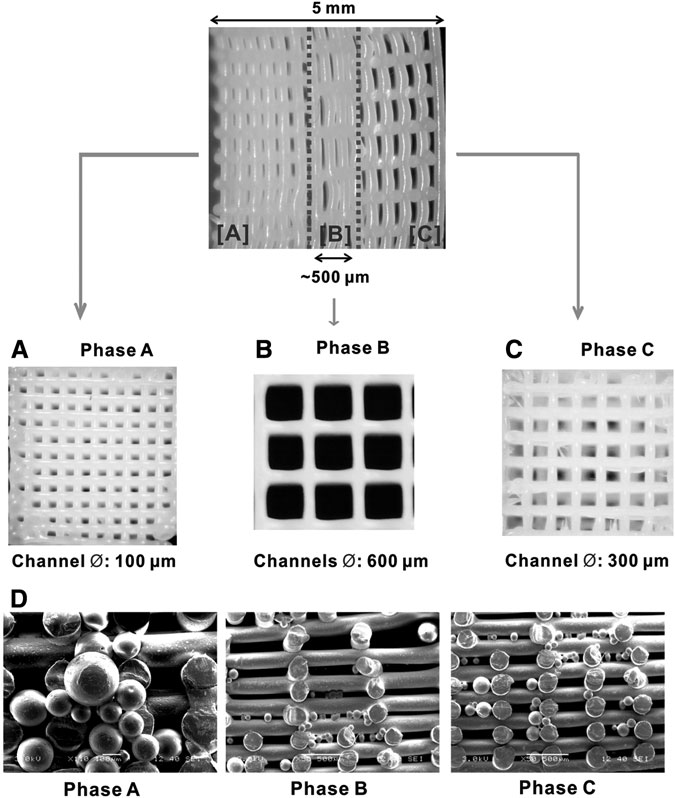
\includegraphics[width=\linewidth, keepaspectratio]{trifase} 
%\caption{}
\label{fig:trifase}
\end{subfigure}
\begin{subfigure}{0.5\textwidth}
\centering
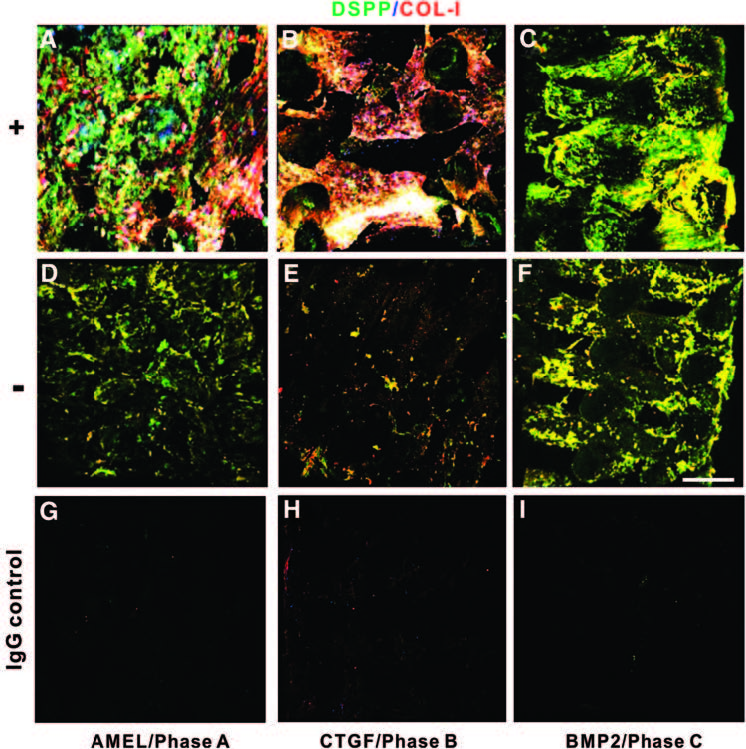
\includegraphics[width=\linewidth, keepaspectratio]{histo}
%\caption{}
\label{fig:histo}
\end{subfigure}
\caption{\textbf{A sinistra}: \emph{scaffold trifase} per la rigenerazione del complesso parodontale con microsfere contenenti fattori di crescita. \emph{\textbf{Phase A}}: scaffold per la rigenerazione del cemento radicolare; \emph{\textbf{Phase B}}: scaffold per la rigenerazione di legamento parodontale; \emph{\textbf{Phase C}}: scaffold per la rigenerazione di osso alveolare. \textbf{A destra}: immagini istologiche di scaffold seminato con DPSC (\emph{Dental Pulp Stem Cell}). \emph{\textbf{Prima riga}} con microsfere contenenti fattori di crescita; \emph{\textbf{seconda riga}} con microsfere vuote. In verde si evidenzia la presenza di DSPP (\emph{Dental SialoPhospho Proteine}, indicante regioni mineralizzate), mentre in rosso è evidenziato il \emph{collagene tipo I}, costituente il legamento parodontale. Barra = \SI {200} {\micro\metre}. Da \emph{Lee et al} \parencite{Reference135}.}
\label{fig:scaffold_trifase}
\end{figure}
\pagebreak

Un altro interessante design per la rigenerazione del complesso parodontale è stato realizzato da Lee \parencite{Reference135}. L'autore ha realizzato una struttura in PCL-HA a diversa porosità e l'ha arricchita con \emph{microsfere} contenenti 3 tre diversi fattori di crescita, uno per ogni regione da rigenerare: \textbf{BMP2} (bone morphogenetic protein 2) per l'osso alveolare, \textbf{CTGF} (connettive tissue growth factor) per il legamento parodontale ed \textbf{Amelogenina} per il cemento radicolare \ref{fig:scaffold_trifase}.\\
Sullo scaffold sono poi state seminate \emph{cellule staminali della polpa dentaria} (DPSC - Dental Pulp Stem Cells). Il costrutto così realizzato è stato quindi impiantato sottocute in delle cavie e prelevato dopo 6 settimane. All'istologia si è notata la presenza di tessuto mineralizzato e fibre di collagene orientate e ordinate che collegano il cemento neoformato all'osso neoformato, in una disposizione molto simile a quella del legamento parodontale (\emph{fibre di Sharpey}) \ref{fig:scaffold_trifase}.

\section{Scaffold design}
Il design di uno scaffold è un passaggio importante, perché bisogna trovare un compromesso tre la forma del difetto, la porosità dello scaffold e le sue proprietà meccaniche, in armonia con i tessuti circostanti. Questo è a maggiormente vero nella realizzazione di scaffold per la rigenerazione del tessuto osseo e del tessuto cartilagineo, in quanto lo scaffold deve fornire adeguate proprietà meccaniche sin dal suo inserimento, ben prima quindi che il tessuto leso si sia rigenerato. Molti design con vari parametri e proprietà sono presenti in letteratura, a sottolineare come ogni tessuto ed ogni condizione funzionale abbia peculiari necessità da soddisfare in fase di progettazione.\\
Vengono qui illustrate delle tecniche base per la generazione di scaffold, che si avvalgono di software attualmente disponibili, senza addentrarsi nella specificità delle caratteristiche dello scaffold, che andranno poi adattate in base al campo di applicazione.

\subsection{Scaffold design in Cura}
Il software che abbiamo usato per lo slicing dei nostri modelli può essere agevolmente utilizzato per realizzare semplici scaffold a partire da un modello base. Utilizzando Cura otterremo il G-Code dello scaffold, ma non sarà possibile ottenere un modello .stl dello stesso.

%\subsubsection{Procedura base}
Per realizzare uno scaffold in Cura dobbiamo partire da un oggetto di base. Usiamo Blender per creare un \textbf{cubo} (è un oggetto di base, reperibile nella schermata principale in \emph{Add}-->\emph{Mesh}-->\emph{Cube}), esportiamolo in formato .stl e importiamolo in Cura.
Caricato il cubo in Cura ne possiamo gestire le dimensioni dal menù sulla sinistra, alla voce \emph{Scale} (si può rimuovere la spunta nella voce \emph{Uniform Scaling} per ridimensionare l'oggetto in maniera non uniforme, ad esempi possiamo creare un parallelepipedo partendo dal cubo). Impostiamo la modalità di visione \emph{Layer View} dal menù in alto a destra; vedremo così la ricostruzione del G-code.\\
Modifichiamo ora le impostazioni di slicing per ottenere uno scaffold. I parametri principali da impostare sono i seguenti:

\begin{itemize}

\item Nel menù \emph{\textbf{Shell}}:
\begin{itemize}
\item \emph{\textbf{Wall Thickness}}: 0; rimuove le pareti laterali del modello
\item \emph{\textbf{Top/Botton Thickness}}: 0; rimuove tetto e base del modello
\end{itemize}

\end{itemize}

Avremo a questo punto un modello senza pareti e ci serviremo dell'infill per gestire i parametri dello scaffold \parencite{Reference138}.

\begin{itemize}
\item Nel menù \emph{\textbf{Infill}}:

\begin{itemize}
\item \textit{\textbf{Infill Pattern}}: \emph{Lines}; questo pattern da luogo all'apposizione di linee deposte in un solo verso, che è perpendicolare al verso delle linee del layer precedente. Questa interposizione di linee alternate da luogo ad una interconnessione completa tra i pori.
\item \emph{\textbf{Infill Line Distance}}: qui possiamo inserire un valore numerico che corrisponderà alla distanza tra linee consecutive in un layer. Utilizziamo questo parametro per il controllo maggiore che ci fornisce sulla geometria rispetto ad Infill Density
\item \emph{\textbf{Infill Line Direction}}: questo parametro ci da il controllo sull'ori\-en\-ta\-men\-to delle linee sul piano XY. Un angolo 0 corrisponde a linee parallele all'asse Y, mentre angolo 90 corrisponde a linee parallele all'asse X. Gli angoli che inseriremo verranno ripetuti per tutta l'altezza dell'oggetto. Per creare layer perpendicolari l'uno all'altro usare [0,90].
Possiamo anche creare più layer di fila con lo stesso angolo; ad esempio [0,0,90,90] ci darà due layer paralleli all'asse Y e due layer perpendicolari allo stesso asse, che si ripeteranno fino al completamento dell'oggetto.Inserire un maggior numero di layer consecutivi orientati nello stesso modo ci permette di controllare la dimensione dei pori sull'asse Z; inoltre permette di avere un maggiore interconnessione tra i pori dello scaffold.
\item \emph{\textbf{Gradual Infill Step}}: definisce il numero di volte in cui la densità dell'infill aumenta fino al valore impostato, con la zona meno densa all'inizio e la più densa alla fine.
\item \emph{\textbf{Gradual Infill Step Height}}: definisce l'altezza dopo la quale si raddoppia la densità dell'infill.
\end{itemize}

\end{itemize}

La regolazione di questi parametri ci permette un discreto controllo sulla geometria dell'infill e quindi dello scaffold \ref{fig:mini_cube_full}. La larghezza di ogni linea (\emph{Line Width}) è dipendente dal diametro dell'ugello, ed è un parametro importante da considerare durante la progettazione. Per garantire l'adesione al piano dell'oggetto durante la stampa è possibile utilizzare \emph{Brim} o \emph{Raft}. \\Con la stessa tecnica qui descritta è possibile ottenere scaffold a partire da modelli anatomici \ref{fig:scaffo_mandibola}.
\begin{figure}[t]
\vspace{-10pt}
	\begin{center}
	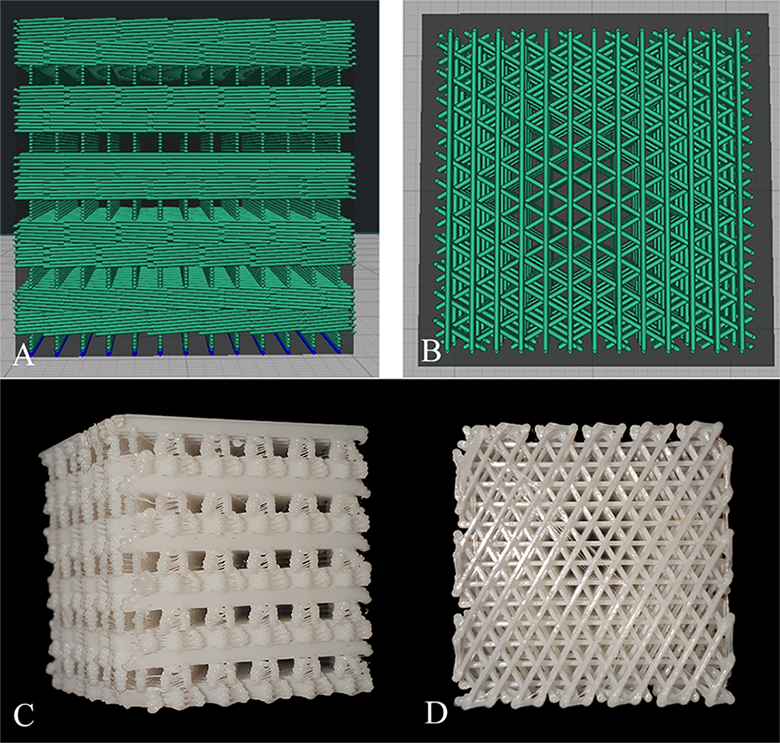
\includegraphics[width=0.9\textwidth, keepaspectratio]{mini_cube_full}
    \caption{\textbf{Scaffold in Cura}, \emph{Layer View}. Cubo 20mm per lato.
\textbf{A}: vista di fronte; \textbf{B}: vista da sopra;
\textbf{C} e \textbf{D}: scaffold stampato in PLA.
\textbf{Layer Height}: 0.2mm
\textbf{Layer Width}: 0.37mm
\textbf{Ugello diametro}: 0.4mm
\textbf{Infill Line Directions}: [0,0,0,0,0,0,60,60,60,60,60\-,60,60,120,120,120,120,120,120,120]
\textbf{Line Infill Distances}: \SI{1.52}{\milli\metre}.}
    \label{fig:mini_cube_full}
	\end{center}
\vspace{-20pt}
\end{figure}

\begin{figure}[t]
\vspace{-10pt}
	\begin{center}
	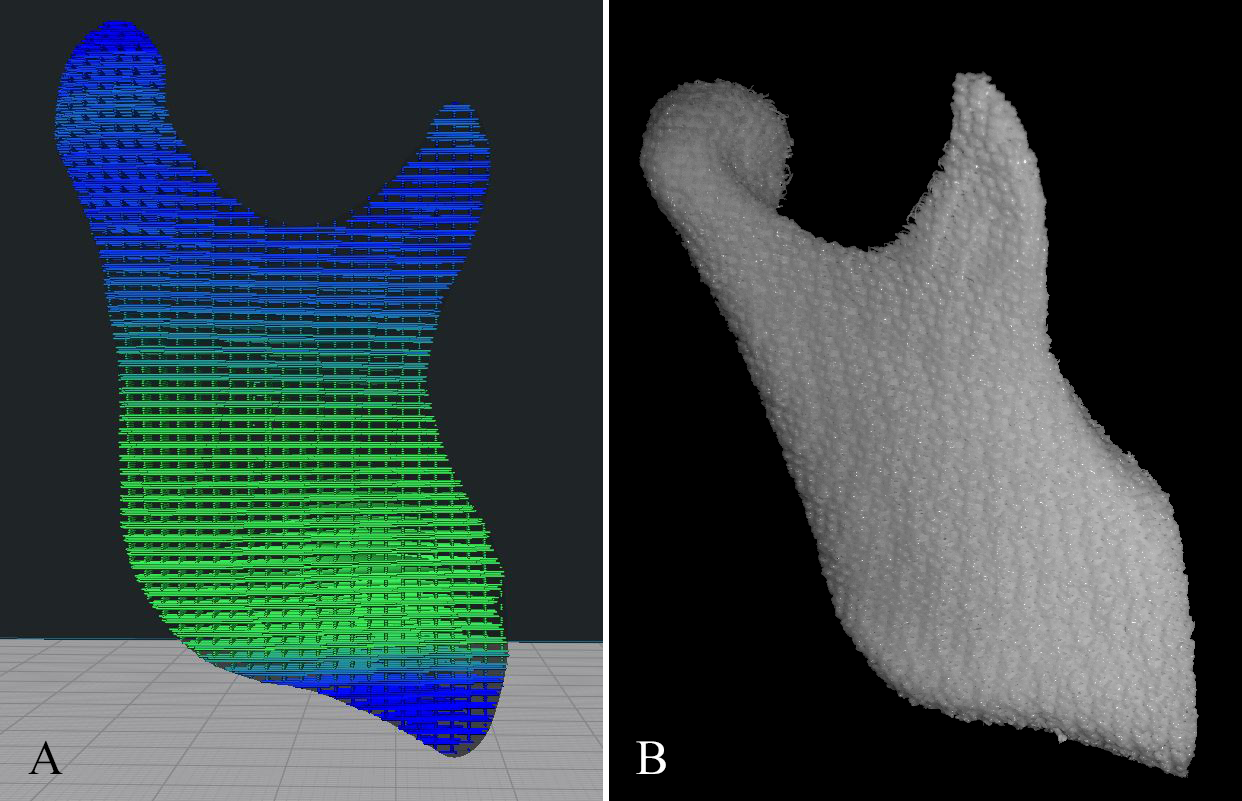
\includegraphics[width=0.9\textwidth, keepaspectratio]{scaffo_mandibola}
    \caption[LoF entry]{Scaffold derivato da un modello di ramo mandibolare.

\textbf{Layer Height}: 0.2mm
\textbf{Layer Width}: 0.37mm
\textbf{Ugello diametro}: 0.4mm
\textbf{Infill Line Directions}: [0,0,0,90,90,90]
\textbf{Line Infill Distances}: 0.8mm}
    \label{fig:scaffo_mandibola}
	\end{center}
\vspace{-20pt}
\end{figure}

